\chapter{Background and Problem Statement}
\label{ch1}

\section{Turbulence ($C_{n}^{2}$) Background}
\subsection{What is Turbulence ($C_{n}^{2}$)?}
Optical (atmospheric) turbulence is caused by naturally occurring small variations in air temperature ($<$ 1\textdegree C) which cause random variations in wind velocity (eddies) which we view as turbulent motion in the atmosphere. The temperature differences cause small differences in atmospheric density and therefore in refractive index. These index changes are moved around by the random variations in wind eddies and can accumulate to cause significant inhomogeneities in the index profile of the atmosphere which can cause the wavefront of a beam to significantly change in propagation. The effects are high spatial frequency beam spreading, low spatial frequency beam wander, and intensity variations (scintillation) \cite{tyson2011principles}. Atmospheric turbulence strength is characterized by the refractive-index structure constant, $C_{n}^{2}$ ($m^{-2/3}$). Turbulence strength is highly variable with season, time of day, geographical location, altitude, and local weather patterns. Generally, $C_{n}^{2}$ varies in value from $1 \times 10^{-12}$ (very strong) to $1 \times 10^{-17}$ (very weak).

Atmospheric turbulence can have many adverse affects on optics in imaging and laser systems. All imaging through a non-negligible distance of the Earth's atmosphere is impacted by atmospheric turbulence, leading to a blurring effect in an image. An example of this is shown in Figure \ref{fig:first_frames}.
\begin{figure}[h!]
	\centering
	\subfloat[Low-strength ($C_{n}^{2}$)\label{fig:first_frames_a}]{
		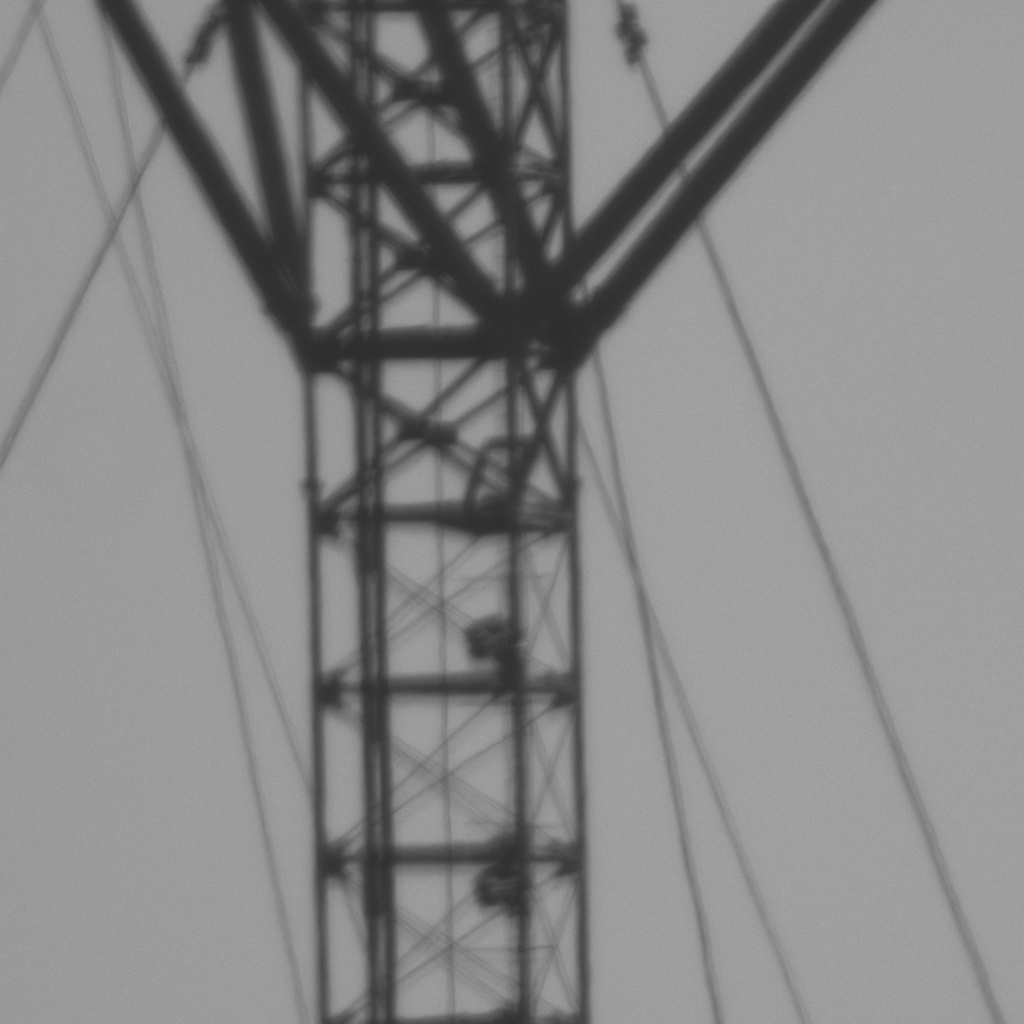
\includegraphics[width=0.49\textwidth]
		{FirstFrame_LowTurb.jpg}
	}
	\subfloat[High-strength ($C_{n}^{2}$)\label{fig:first_frames_b}]{
		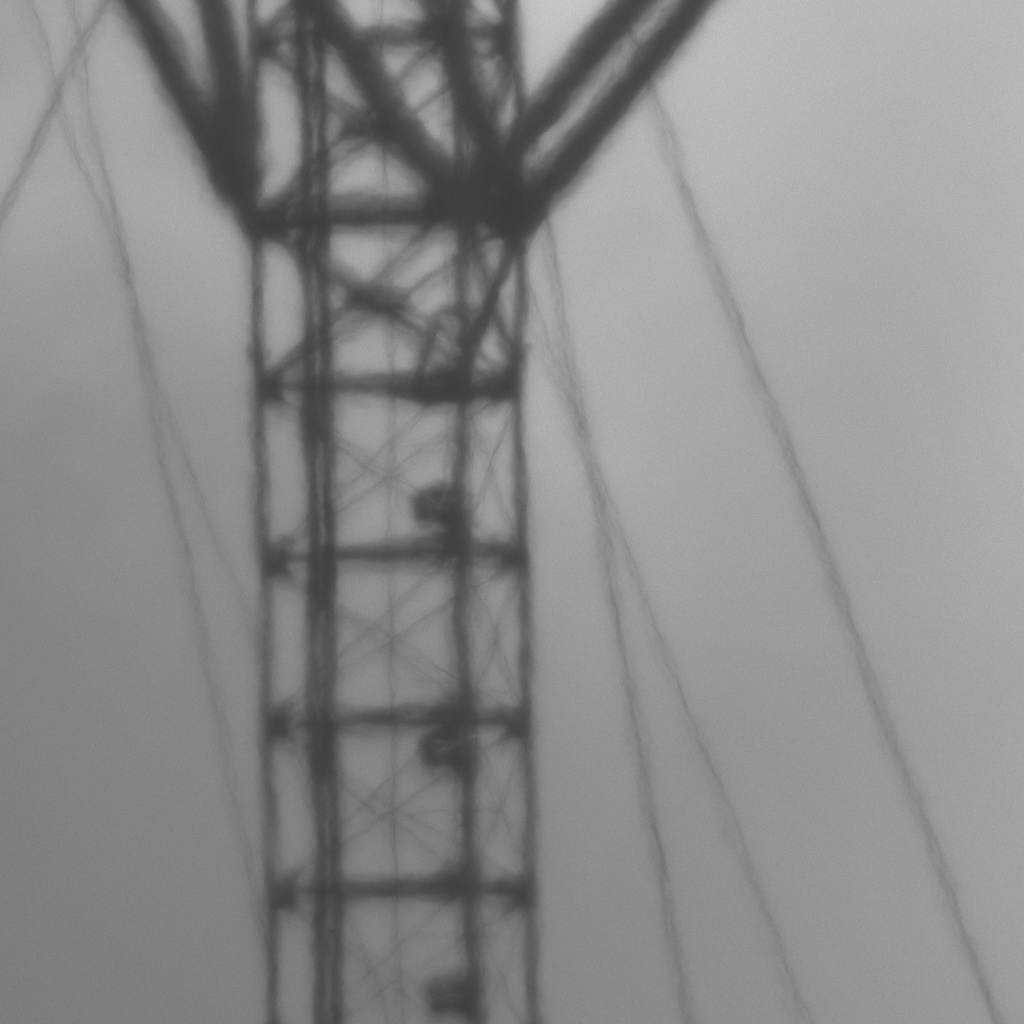
\includegraphics[width=0.49\textwidth]
		{FirstFrame_HighTurb.jpg}
	}
	\hfill
	\caption{Effect of low-strength and high-strength $C_{n}^{2}$ conditions.}
	\label{fig:first_frames}
\end{figure}
Both images in Figure \ref{fig:first_frames} are of the same target on the same day but during low-strength turbulence (left) and high-strength turbulence (right) conditions. There are many developed and developing technologies which are highly impacted by the impact of atmospheric turbulence.

In imaging applications, the image degradation in Figure \ref{fig:first_frames_b} due to strong turbulence can significantly impact feature extraction and target recognition. The twinkling of celestial objects in the night sky is due to atmospheric turbulence. Observatories (astronomy) are frequently built at high altitude geographical locations in part to avoid light pollution, but also to reduce amount of turbulence degradation by shortening the distance the incoming light must propagate through the atmosphere. In laser propagation applications, the degradation of the wavefront can significantly reduce the power of a beam on the target from a high energy laser (HEL) weapon system, or disrupt the transfer of signal in optical communication.

Atmospheric turbulence is important to measure and model because the atmospheric turbulence impact can be compensated with adaptive optics (AO). The strength of the atmospheric turbulence is proportional to the amount of adaptive optics compensation needed to correct for the aberrations. Using astronomy as an example, the basic components of an adaptive optics system consists of a wavefront sampler, a wavefront sensor (WFS), a corrector such as a deformable mirror, and a control computer to perform real-time numerical calculations. Light from an astronomical object is captured by the optical system consisting of a telescope and imager (camera). Part of the light is sampled by the WFS and this data is sent to the computer to calculate the necessary corrections in the deformable mirror to sharpen the image \cite{tyson2011principles}. A similar system exists for a laser propagation setup. Another application of the measurement of turbulence an optical system which requires parameter tuning at a specific strength of $C_{n}^{2}$ for further experimentation or use. Finally, the use of a laser weapon system might be best for turbulence conditions weaker than a specific strength so knowledge of the current conditions can decide whether to use the laser system or traditional weapons.

\subsection{State of Turbulence ($C_{n}^{2}$) Modeling}
There is no theoretical (physical) model for turbulence which is accurate for the many cases, but many have been developed for specific cases. One such model is the Hufnagel-Valley boundary model calculates $C_{n}^{2}$ as a function of altitude \cite{Valley:80}. Another is the submarine laser communications (SLC)-Night model which associates $C_{n}^{2}$ strengths with specific altitude ranges \cite{tyson2011principles}.

Another approach to modeling turbulence ($C_{n}^{2}$), specifically at the surface level, is by the use of machine learning. This approach acts as a surrogate model of the relationship between the local environmental (weather) and $C_{n}^{2}$ measurements. Typical weather measurements are air temperature, pressure, relative humidity or dew point, wind speed and direction, solar irradiance, and time-correlated atmospheric turbulence ($C_{n}^{2}$) typically with a scintillometer \cite{Jellen:20, Su:20, Wang:2014}. The machine learning approach primary employs the artificial neural network (ANN) in a multi-layer perceptron (MLP) optimized by a gradient descent algorithm \cite{Su:20, Wang:2014}. \textbf{TALK ABOUT MORE LITERATURE?}

This type of approach associates a set of environmental (weather) measurements with a time-correlated $C_{n}^{2}$ measurement and is most useful as a surrogate model to predict $C_{n}^{2}$ for comparison with measurements. This technique illustrates the capability of a model, but from a utility perspective is only useful if current $C_{n}^{2}$ measurements are desired but a sensor is not deployed. A more useful model \emph{forecasts} future $C_{n}^{2}$ instead of making time-correlated predictions. One approach to this is to train a regression model on time-correlated weather and $C_{n}^{2}$ measurements, then apply it to weather forecasts from a numerical weather prediction (NWP) data source to yield a $C_{n}^{2}$ forecast.

The work in this thesis develops a novel machine learning approach to forecast future daytime $C_{n}^{2}$ conditions from \emph{prior} environmental (weather) and $C_{n}^{2}$ measurements. Deep learning is used to create a low-altitude model capable of forecasting 4 hours of future daytime $C_{n}^{2}$ conditions with estimates every 30 minutes using no more than 16 hours of prior environmental measurements. This technique is ideal for any application that uses future $C_{n}^{2}$ predictions and bypasses the need to download and format NWP data for model inference.

\section{Thesis Overview}
This section provides a brief chapter-by-chapter overview of the work in this thesis.

\subsection{Machine Learning Modeling Review (Ch. 2)}
Chapter \ref{ch2} steps through a review of machine learning modeling. First, the basics of model training and testing is summarized. Next, the fundamental machine learning architectures used throughout this work are described in detail. Finally, other vital components to machine learning modeling such as optimization are reviewed.

\subsection{Dataset (Ch. 3)}
Chapter \ref{ch3} first summarizes the weather and $C_{n}^{2}$ data sources and their spatial relationship to each other. Chapter \ref{ch3} then details the data preprocessing techniques including confidence filtering, window averaging, and interpolating. Finally, the methodology is described to format the data into model input/output pairs and parse into train, validation, and test datasets.

\subsection{Grid Search (Ch. 4)}
Chapter \ref{ch4} details the technique used to find the best architecture and parameters to best forecast $C_{n}^{2}$: the grid search. A statistical test, the \textit{Student's t-test}, is described then employed as a significance test of the grid search results. The top performing models in the grid search are then compared and a single model is selected.

\subsection{Test Dataset Model Evaluation (Ch. 5)}
Chapter \ref{ch5} applies the selected model to the test dataset and illustrates performance. This Chapter then details an analysis on the overall model performance to illustrate general model capabilities, and then analyzes three specific forecasts to understand why the model performs well and poorly in specific scenarios.

\subsection{Summary and Future Work (Ch. 6)}
Chapter \ref{ch6} summarizes this thesis and details items for future work encountered throughout this effort.